\documentclass[../Cours.tex]{subfiles}

\begin{document}
\clearpage
\thispagestyle{empty}

\setcounter{DS}{1}

\color{black}
\nomPrenom{}
\titreDS

\begin{questions}
    \EXERCICETITRE{3}{DISTANCE D'ARRÊT}
    \bionic[0.4]{Lorsque le conducteur d'un véhicule perçoit un obstacle et veut freiner, il va d'abord avoir un temps de réaction d'une seconde ; cette distance est appelée distance de réaction. Puis, il va appuyer sur la pédale de frein, et la voiture va freiner sur une certaine distance appelée distance de freinage.\\
    La distance d'arrêt est la somme de la distance de réaction et de la distance de freinage.}\\    

    \question Si une voiture roule à \qty{20}{\metre\per\second}, quelle est sa distance de réaction ? \caseReponse{2}

    \begin{center}
    \begin{tikzpicture}
        \node[anchor=west] at (-2,1.5) {Pour calculer la distance de freinage, on utilise la formule :};
        \node at (2.5,-0.5) {$D_f = \dfrac{v^2}{2 \times g \times a}$};
        \node[anchor=west] at (6.5,0) {$v$ est la vitesse (en \unit{\metre\per\second})};
        \node[anchor=west] at (6.5,-0.6) {$g = 10$};
        \node[anchor=west] at (6.5,-1.2) {$a = 0,8$ sur route sèche, $a = 0,6$ sur route mouillée};
        \draw[dashed] (-2,1.8) rectangle (16,-2);
    \end{tikzpicture}
    \end{center}
    \question Si une voiture roule à \qty{20}{\metre\per\second} sur route mouillée, quelle est sa distance de freinage ? \caseReponse{2}
    \question En déduire sa distance d'arrêt. \caseReponse{2}

    \clearpage
    \EXERCICETITRE{4}{Suite de figures}
    \begin{center}
    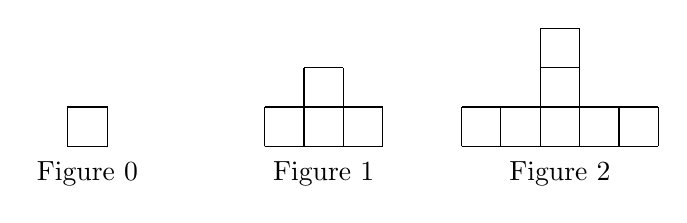
\begin{tikzpicture}[scale=0.5]
        \draw (0,0) rectangle (1,1);
        \node at (0.5,-0.7) {Figure 0};
        \draw (5,0) grid (8,1);
        \draw (6,0) grid (7,2);
        \node at (6.5,-0.7) {Figure 1};
        \draw (10,0) grid (15,1);
        \draw (12,0) grid (13,3);
        \node at (12.5,-0.7) {Figure 2};
    \end{tikzpicture}
    \end{center}

    En poursuivant cette suite de figures, combien y aura-t-il de carrés...
    \question pour la figure 3 ?
    \question pour la figure 10 ?
    \question pour la figure 100 ?
    \question pour la figure $n$ ?

    \caseReponse{4}

    \EXERCICETITRE{4}{Dame blanche}
    \bionic[0.4]{Une dame blanche est un dessert composée de deux boules de glace à la vanille et d'une boule de glace au chocolat.\\ Dans un restaurant, le gérant achète} $\qty{500}{\litre}$ \bionic[0.4]{de glace au chocolat et}  $\qty{1000}{\litre}$ \bionic[0.4]{de glace à la vanille. }\\

    \question Sachant que toutes les boules de glaces ont pour rayon $\qty{5}{cm}$, quel est le volume d'une boule de glace ? (Rappel : $V_{\mbox{boule}} = \frac{4}{3} \pi \times \mbox{rayon}^3$)

    \caseReponse{2}
    
    \question Combien de dames blanches pourra-t-on faire dans ce restaurant ?

    \caseReponse{2}

    \clearpage

    \EXERCICETITRE{4}{THALÈS}

    \begin{center}
    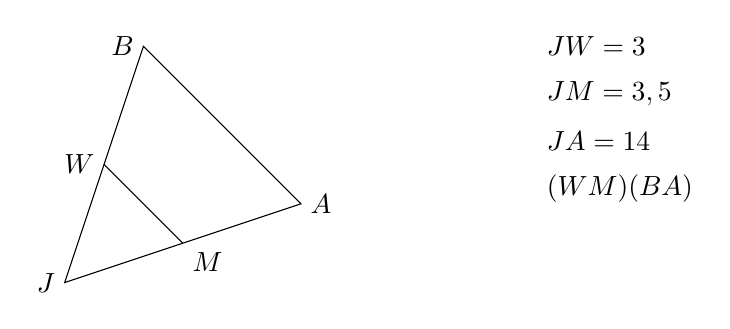
\begin{tikzpicture}
        \draw (0,0) node[left]{$J$} -- (1,3) node[left]{$B$} -- (3,1) node[right]{$A$} -- cycle;
        \draw (0.5,1.5) node[left]{$W$} -- (1.5,0.5) node[below right]{$M$};
        \node[anchor=west] at (6,3) {$JW = 3$};
        \node[anchor=west] at (6,2.4) {$JM = 3,5$};
        \node[anchor=west] at (6,1.8) {$JA = 14$};
        \node[anchor=west] at (6,1.2) {$(WM) \paral (BA)$};
    \end{tikzpicture}
    \end{center}

    \question Déterminer $JB$

    \caseReponse{5}

    \EXERCICETITRE{5}{THALÈS ET PYTHAGORE}

    $ABR$ est un triangle rectangle $B$, tel que $AB = 17$ et $BR = 19$. \\
    Placer $I$ sur $[AB]$ tel que $AI=3$. \\
    On trace une droite $(d)$ perpendiculaire à $(AB)$ passant par $I$, coupant $(AR)$ en $J$.

    \question Calculer $AR$

    \caseReponse{7}

    \clearpage
    \question Calculer $IJ$

    \caseReponse{6}

    \EXERCICETITRE{(bonus) 2}{AVEC DES $x$}

    $ABC$ est un triangle rectangle en $B$ tel que $AB = 3x$ et $BC = 4x$.

    \question Calculer $AC$
    \question En déduire les dimensions de 3 triangles rectangles, en évaluant $x$ avec des valeurs quelconques.

    \caseReponse{7}
    
\end{questions}
\end{document}